

\tikzset{every picture/.style={line width=0.75pt}} %set default line width to 0.75pt        

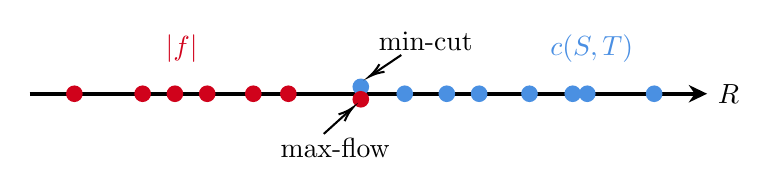
\begin{tikzpicture}[x=0.5pt,y=0.5pt,yscale=-1,xscale=1]
%uncomment if require: \path (0,126); %set diagram left start at 0, and has height of 126

%Straight Lines [id:da6845720994983642] 
\draw [line width=1.5]    (7,59) -- (492.5,59) ;
\draw [shift={(496.5,59)}, rotate = 180] [fill={rgb, 255:red, 0; green, 0; blue, 0 }  ][line width=0.08]  [draw opacity=0] (13.4,-6.43) -- (0,0) -- (13.4,6.44) -- (8.9,0) -- cycle    ;
%Shape: Circle [id:dp5839925944461984] 
\draw  [color={rgb, 255:red, 74; green, 144; blue, 226 }  ,draw opacity=1 ][fill={rgb, 255:red, 74; green, 144; blue, 226 }  ,fill opacity=1 ] (241,54) .. controls (241,51.1) and (243.35,48.75) .. (246.25,48.75) .. controls (249.15,48.75) and (251.5,51.1) .. (251.5,54) .. controls (251.5,56.9) and (249.15,59.25) .. (246.25,59.25) .. controls (243.35,59.25) and (241,56.9) .. (241,54) -- cycle ;
%Shape: Circle [id:dp34886579289539754] 
\draw  [color={rgb, 255:red, 208; green, 2; blue, 27 }  ,draw opacity=1 ][fill={rgb, 255:red, 208; green, 2; blue, 27 }  ,fill opacity=1 ] (188.65,59) .. controls (188.65,56.1) and (191,53.75) .. (193.9,53.75) .. controls (196.8,53.75) and (199.15,56.1) .. (199.15,59) .. controls (199.15,61.9) and (196.8,64.25) .. (193.9,64.25) .. controls (191,64.25) and (188.65,61.9) .. (188.65,59) -- cycle ;
%Shape: Circle [id:dp4135235202894928] 
\draw  [color={rgb, 255:red, 208; green, 2; blue, 27 }  ,draw opacity=1 ][fill={rgb, 255:red, 208; green, 2; blue, 27 }  ,fill opacity=1 ] (34,59) .. controls (34,56.1) and (36.35,53.75) .. (39.25,53.75) .. controls (42.15,53.75) and (44.5,56.1) .. (44.5,59) .. controls (44.5,61.9) and (42.15,64.25) .. (39.25,64.25) .. controls (36.35,64.25) and (34,61.9) .. (34,59) -- cycle ;
%Shape: Circle [id:dp20365687038540725] 
\draw  [color={rgb, 255:red, 208; green, 2; blue, 27 }  ,draw opacity=1 ][fill={rgb, 255:red, 208; green, 2; blue, 27 }  ,fill opacity=1 ] (83.33,59) .. controls (83.33,56.1) and (85.68,53.75) .. (88.58,53.75) .. controls (91.48,53.75) and (93.83,56.1) .. (93.83,59) .. controls (93.83,61.9) and (91.48,64.25) .. (88.58,64.25) .. controls (85.68,64.25) and (83.33,61.9) .. (83.33,59) -- cycle ;
%Shape: Circle [id:dp001936474221955753] 
\draw  [color={rgb, 255:red, 208; green, 2; blue, 27 }  ,draw opacity=1 ][fill={rgb, 255:red, 208; green, 2; blue, 27 }  ,fill opacity=1 ] (106.66,59) .. controls (106.66,56.1) and (109.01,53.75) .. (111.91,53.75) .. controls (114.81,53.75) and (117.16,56.1) .. (117.16,59) .. controls (117.16,61.9) and (114.81,64.25) .. (111.91,64.25) .. controls (109.01,64.25) and (106.66,61.9) .. (106.66,59) -- cycle ;
%Shape: Circle [id:dp8083671983789567] 
\draw  [color={rgb, 255:red, 208; green, 2; blue, 27 }  ,draw opacity=1 ][fill={rgb, 255:red, 208; green, 2; blue, 27 }  ,fill opacity=1 ] (129.99,59) .. controls (129.99,56.1) and (132.34,53.75) .. (135.24,53.75) .. controls (138.14,53.75) and (140.49,56.1) .. (140.49,59) .. controls (140.49,61.9) and (138.14,64.25) .. (135.24,64.25) .. controls (132.34,64.25) and (129.99,61.9) .. (129.99,59) -- cycle ;
%Shape: Circle [id:dp9076802577362922] 
\draw  [color={rgb, 255:red, 208; green, 2; blue, 27 }  ,draw opacity=1 ][fill={rgb, 255:red, 208; green, 2; blue, 27 }  ,fill opacity=1 ] (163.32,59) .. controls (163.32,56.1) and (165.67,53.75) .. (168.57,53.75) .. controls (171.47,53.75) and (173.82,56.1) .. (173.82,59) .. controls (173.82,61.9) and (171.47,64.25) .. (168.57,64.25) .. controls (165.67,64.25) and (163.32,61.9) .. (163.32,59) -- cycle ;
%Shape: Circle [id:dp4236178447115101] 
\draw  [color={rgb, 255:red, 208; green, 2; blue, 27 }  ,draw opacity=1 ][fill={rgb, 255:red, 208; green, 2; blue, 27 }  ,fill opacity=1 ] (241,63) .. controls (241,60.1) and (243.35,57.75) .. (246.25,57.75) .. controls (249.15,57.75) and (251.5,60.1) .. (251.5,63) .. controls (251.5,65.9) and (249.15,68.25) .. (246.25,68.25) .. controls (243.35,68.25) and (241,65.9) .. (241,63) -- cycle ;
%Shape: Circle [id:dp5050758022328539] 
\draw  [color={rgb, 255:red, 74; green, 144; blue, 226 }  ,draw opacity=1 ][fill={rgb, 255:red, 74; green, 144; blue, 226 }  ,fill opacity=1 ] (272.76,59) .. controls (272.76,56.1) and (275.11,53.75) .. (278.01,53.75) .. controls (280.91,53.75) and (283.26,56.1) .. (283.26,59) .. controls (283.26,61.9) and (280.91,64.25) .. (278.01,64.25) .. controls (275.11,64.25) and (272.76,61.9) .. (272.76,59) -- cycle ;
%Shape: Circle [id:dp8576227272464049] 
\draw  [color={rgb, 255:red, 74; green, 144; blue, 226 }  ,draw opacity=1 ][fill={rgb, 255:red, 74; green, 144; blue, 226 }  ,fill opacity=1 ] (303.14,59) .. controls (303.14,56.1) and (305.49,53.75) .. (308.39,53.75) .. controls (311.29,53.75) and (313.64,56.1) .. (313.64,59) .. controls (313.64,61.9) and (311.29,64.25) .. (308.39,64.25) .. controls (305.49,64.25) and (303.14,61.9) .. (303.14,59) -- cycle ;
%Shape: Circle [id:dp40578843932984965] 
\draw  [color={rgb, 255:red, 74; green, 144; blue, 226 }  ,draw opacity=1 ][fill={rgb, 255:red, 74; green, 144; blue, 226 }  ,fill opacity=1 ] (326.52,59) .. controls (326.52,56.1) and (328.87,53.75) .. (331.77,53.75) .. controls (334.67,53.75) and (337.02,56.1) .. (337.02,59) .. controls (337.02,61.9) and (334.67,64.25) .. (331.77,64.25) .. controls (328.87,64.25) and (326.52,61.9) .. (326.52,59) -- cycle ;
%Shape: Circle [id:dp2060326184335437] 
\draw  [color={rgb, 255:red, 74; green, 144; blue, 226 }  ,draw opacity=1 ][fill={rgb, 255:red, 74; green, 144; blue, 226 }  ,fill opacity=1 ] (362.9,59) .. controls (362.9,56.1) and (365.25,53.75) .. (368.15,53.75) .. controls (371.05,53.75) and (373.4,56.1) .. (373.4,59) .. controls (373.4,61.9) and (371.05,64.25) .. (368.15,64.25) .. controls (365.25,64.25) and (362.9,61.9) .. (362.9,59) -- cycle ;
%Shape: Circle [id:dp7156703955132185] 
\draw  [color={rgb, 255:red, 74; green, 144; blue, 226 }  ,draw opacity=1 ][fill={rgb, 255:red, 74; green, 144; blue, 226 }  ,fill opacity=1 ] (394.16,59) .. controls (394.16,56.1) and (396.51,53.75) .. (399.41,53.75) .. controls (402.31,53.75) and (404.66,56.1) .. (404.66,59) .. controls (404.66,61.9) and (402.31,64.25) .. (399.41,64.25) .. controls (396.51,64.25) and (394.16,61.9) .. (394.16,59) -- cycle ;
%Shape: Circle [id:dp5714468634699819] 
\draw  [color={rgb, 255:red, 74; green, 144; blue, 226 }  ,draw opacity=1 ][fill={rgb, 255:red, 74; green, 144; blue, 226 }  ,fill opacity=1 ] (404.66,59) .. controls (404.66,56.1) and (407.01,53.75) .. (409.91,53.75) .. controls (412.81,53.75) and (415.16,56.1) .. (415.16,59) .. controls (415.16,61.9) and (412.81,64.25) .. (409.91,64.25) .. controls (407.01,64.25) and (404.66,61.9) .. (404.66,59) -- cycle ;
%Shape: Circle [id:dp338221725625915] 
\draw  [color={rgb, 255:red, 74; green, 144; blue, 226 }  ,draw opacity=1 ][fill={rgb, 255:red, 74; green, 144; blue, 226 }  ,fill opacity=1 ] (453,59) .. controls (453,56.1) and (455.35,53.75) .. (458.25,53.75) .. controls (461.15,53.75) and (463.5,56.1) .. (463.5,59) .. controls (463.5,61.9) and (461.15,64.25) .. (458.25,64.25) .. controls (455.35,64.25) and (453,61.9) .. (453,59) -- cycle ;
%Straight Lines [id:da046923477941067104] 
\draw    (219.5,88) -- (239.02,70.34) ;
\draw [shift={(240.5,69)}, rotate = 497.86] [color={rgb, 255:red, 0; green, 0; blue, 0 }  ][line width=0.75]    (10.93,-3.29) .. controls (6.95,-1.4) and (3.31,-0.3) .. (0,0) .. controls (3.31,0.3) and (6.95,1.4) .. (10.93,3.29)   ;
%Straight Lines [id:da008869050799750533] 
\draw    (275.5,31) -- (254.16,45.38) ;
\draw [shift={(252.5,46.5)}, rotate = 326.02] [color={rgb, 255:red, 0; green, 0; blue, 0 }  ][line width=0.75]    (10.93,-3.29) .. controls (6.95,-1.4) and (3.31,-0.3) .. (0,0) .. controls (3.31,0.3) and (6.95,1.4) .. (10.93,3.29)   ;

% Text Node
\draw (502,50) node [anchor=north west][inner sep=0.75pt]   [align=left] {$\displaystyle R$};
% Text Node
\draw (103,14) node [anchor=north west][inner sep=0.75pt]   [align=left] {$\displaystyle \textcolor[rgb]{0.82,0.01,0.11}{| f| }$};
% Text Node
\draw (381,14) node [anchor=north west][inner sep=0.75pt]   [align=left] {$\displaystyle \textcolor[rgb]{0.29,0.56,0.89}{c( S,T)}$};
% Text Node
\draw (186,89) node [anchor=north west][inner sep=0.75pt]   [align=left] {\textcolor[rgb]{0,0,0}{max-flow}};
% Text Node
\draw (257,12) node [anchor=north west][inner sep=0.75pt]   [align=left] {\textcolor[rgb]{0,0,0}{min-cut}};


\end{tikzpicture}

